\chapter{Introducing Taggle}


\label{chap:taggle}
\ifpdf
    \graphicspath{{Chapters/Taggle/TaggleFigs/PNG/}{Chapters/Taggle/TaggleFigs/PDF/}{Chapters/Taggle/TaggleFigs/}}
\else
    \graphicspath{{Chapters/Taggle/TaggleFigs/EPS/}{Chapters/Taggle/TaggleFigs/}}
\fi  

This chapter describes the details of Taggle's implementation of tag cloud visualisation for software engineering data.  We first review the Taggle data model and describe how data is transformed to fit into this model. We then define the visual encodings and layout algorithm used to render the transformed data for display.

\section{Data Model and Transformation}

We implemented an interactive tag cloud visualisation tool in Java using the Java 2D API for graphics and imaging. Source data for Taggle may be generated externally and provided in an XML format conforming to a DTD. There are a variety of tools/methods which can produce software metric data from source code (such as that proposed by \citep{irwin03}, and see \S\vref{appdx:tools} for a list of available plugins, software analysis platforms and frameworks/tools that can generate metric data). Most of these tools can output data into a CSV or XML format (Table~\vref{table:outputformat}). We produced a tool to convert CSV formatted data to the Taggle XML format, this has also proved useful for conversion of generic datasets that may easily be obtained from external sources. Tools which produce XML formatted output only may also be transformed (using XSLT for example). Typical workflow involved in generating a tag cloud is shown in Figure~\vref{fig:workflow}.

\begin{figure} [h!]
  	\centering
   	\includegraphics[width=60mm]{workflow.png}
  	\caption{Workflow}
	\label{fig:workflow}
\end{figure}

The Taggle XML format specifies tags representing such things as measurement scales (such as nominal, ordinal and ratio) and relationships. Visual mapping and constraints for each field can then be specified via the GUI. Once the constraints of the visual property are set, a relative weighting for each tag is calculated according to the rank of the measurement. The calculation of rank is dependent on the measurement scale type. 

A ``bucket'' ranking value is calculated for ordinal types: $\omega=\rho\diagup\eta$ where $\rho$ is the tag rank in the ordered set, $\eta$ is the total number of tags, and $\omega$ is the resulting weighting, such that $0 \leq \omega \leq 1$. 

For ratio types, we take into account the distance between values on a scale using the following formula: $\omega=(\alpha-min\xi)\diagup (max\xi - min\xi)$ where $\alpha$ is the measurement value, $min\xi$ and $max\xi$ are the lowest and highest values for all measurements for the specified field, and $\omega$ is the resulting weighting, such that $0 \leq \omega \leq 1$. If the setting is specified by the user, $\omega$ is then converted to its hyperbolic tangent. 

These weightings (based on the measurement value) are used to calculate the value of the visual property for an individual tag, between the user defined constraints for a visual property (for example minimum and maximum font sizes).

As an example, consider the tag cloud in Figure~\vref{fig:activemqcamel}: the XML source file contained quality metrics from a subproject of open source project  ActiveMQ, the metrics were of the Chidamber and Kemerer suite generated by the CKJM toolkit. These were originally produced in space separated text format, converted to CSV by OpenOffice, and then converted to the Taggle XML format by our conversion tool. In the GUI, the nominal field ``Class'' was mapped to the tag text (Arial font), the ratio field ``LCOM'' was mapped to the tag ordering property and the font size property (spanning from 20pt to 35pt), and the ratio field ``CBO'' was mapped to a background colour range from black to red. The tags have been positioned according to a simple tag cloud layout algorithm ``typewriter'', where the tags are mapped sequentially left to right, top to bottom.

\begin{figure} [h!]
  	\centering
   	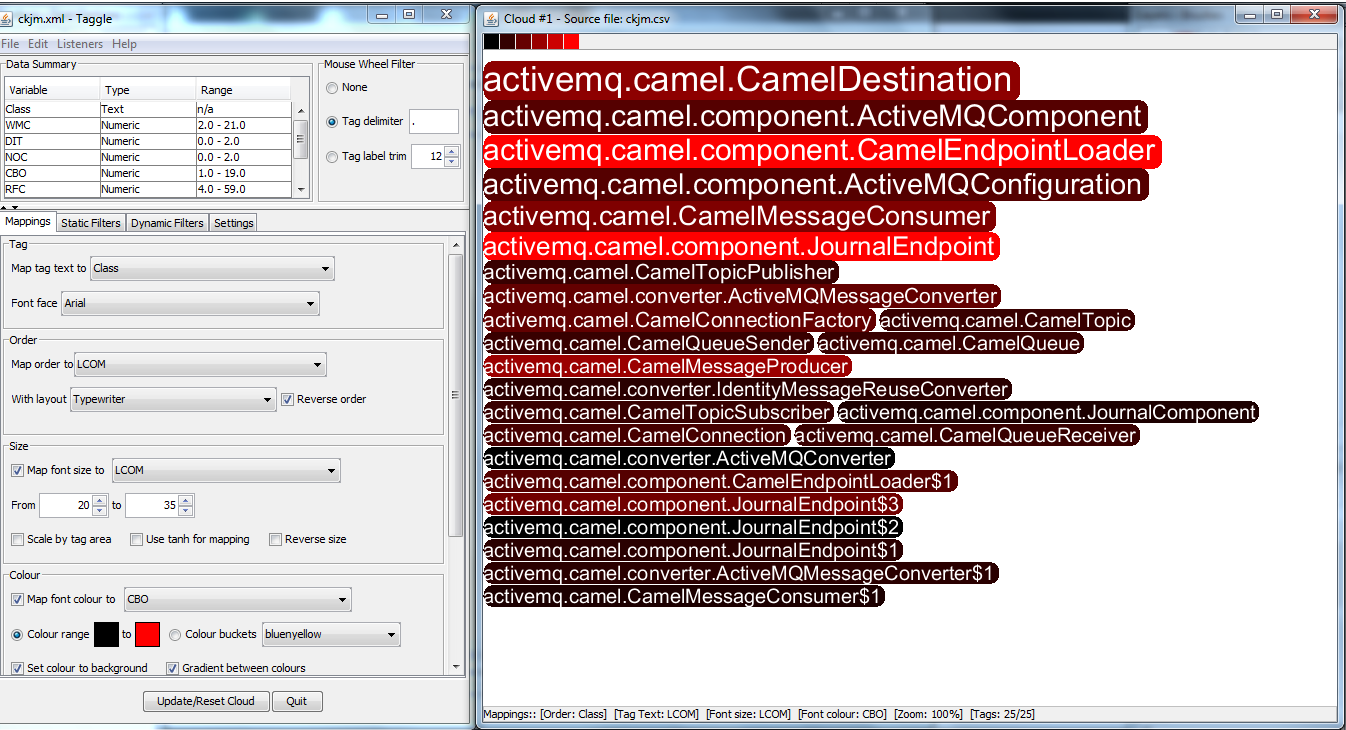
\includegraphics{activemqcamel.png}
  	\caption{\textit{A tag cloud generated by Taggle depicting a subproject of ActiveMQ with metrics derived from CKJM. Visual mapping interface is on the left.}}
	\label{fig:activemqcamel}
\end{figure}

Default values for the visual mappings and other settings for Taggle can be controlled using an external XML file.

 
\section{Rich Interaction}

Taggle includes a number of interactive features to enable rich data exploration. 

\subsection{Dealing with large scale data}

Link to chap 3.

Overview. Details on demand. Follow with filtering. Dynamic querying. Zoom.
Constrained by label length - apply dynamic mouse wheel filtering and label trimming.

\subsection{Identifying skewed data}

Link to chap 3.

\subsection{Identifying outliers}

Link to chap 3.

\subsection{Relationships}

Relationship highlighting. Listeners. Subclouds and linking.

\section{Layout}

\section{Visual Encoding}

The user is supported in the choice of appropriate mappings for the tag cloud by a data summary screen shown in a resizeable pane at the top of the GUI \textemdash for an example see Figure~\vref{fig:datasummary}. Each field in the data file is shown along with data type (text, numeric or categorical) and a range of values. These data types are determined programmatically, fields are labelled categorical when the value ranges correspond to a certain maximum distinct number of values (the actual number is controlled via a setting). Categorical variables are used predominantly in colour mappings (\S\vref{colourmappings}). The data summary panel was included by request from a heuristic evaluation (see Chapter~\vref{chap:heuristiceval}).

\begin{figure} [h!]
  	\centering
   	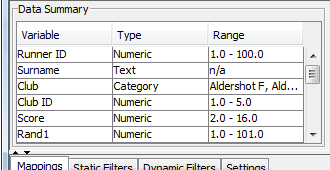
\includegraphics[scale=0.80]{datasummary2.png}
  	\caption{\textit{Closeup of an example data summary panel containing all types of fields}}
	\label{fig:datasummary}
\end{figure}

\subsection{Tag}

The user is free to select any field to map to the tag text, including numeric types. 

The font face dropdown box is pre-populated with fonts that are installed on the machine running Taggle. However, studies have shown that reading speed is best when users are presented with familiar fonts such as Arial, Helvetica and Times New Roman\citep[pg 106, chap 11:7][]{usability06}. In Taggle, the user is free to select any installed font but the familiar fonts mentioned (or the equivalent depending on the operating system and installed word processing software) are highlighted for selection by the user at the top of the dropdown box, separated by a divider (see Figure~\vref{fig:fontfamily}).

\begin{figure} [h!]
  	\centering
   	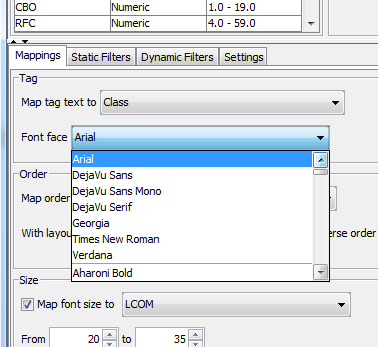
\includegraphics[scale=0.50]{fontfamily.png}
  	\caption{\textit{Prompting selection of familiar fonts.}}
	\label{fig:fontfamily}
\end{figure}

\subsection{Order}

If the order visual property is mapped to a field containing textual data, ordering of the tags is determined alphabetically, otherwise tags are ranked by their numerical value. The selected ordering can be reversed with the ``reverse order'' checkbox and updating the tag cloud.

The user can select an appropriate layout from typewriter, spiral or force directed (defaulting to the simplest layout, typewriter).

\subsection{Size}

Research has indicated slower reading performance for smaller font size \citep[pg 107, chap 11:8][]{usability06}, so there are constraints on the minimum font size to be set to no less than 9pt.

Immediately distinguishable size variations are thought to be no more than about five when data points are placed separately on the display \citep{bertin83}. If data points are adjacent then size variations can be seen up to about 40 or 50. In Taggle, we can order tags by the same field mapped to font size. In Figure~\vref{fig:fontsize}a font size and order are both mapped to field Score. We know immediately now for example, that tag ``Small'' has a higher score than tag ``Firth''. When font size and order are not mapped to the same data field it may not be so obvious. You may need to pull out the relevant tags and put next to one another for easier comparision \textemdash see Figure~\vref{fig:fontsize}b. Alternatively you can hover over the tags and view the actual score measurement details in the pop-up context label.

\begin{figure}[h!]
\begin{subfigure}{\textwidth}
	\centering
	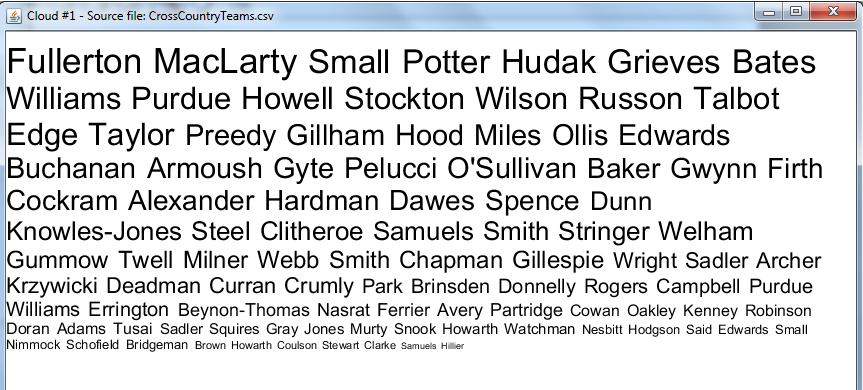
\includegraphics[scale=0.50]{adjacentfont.png}
	\label{fig:adjacentfont}
	\caption{\textit{Order and font size mappings are the same}}
\end{subfigure}
\begin{subfigure}{\textwidth}
  \centering
  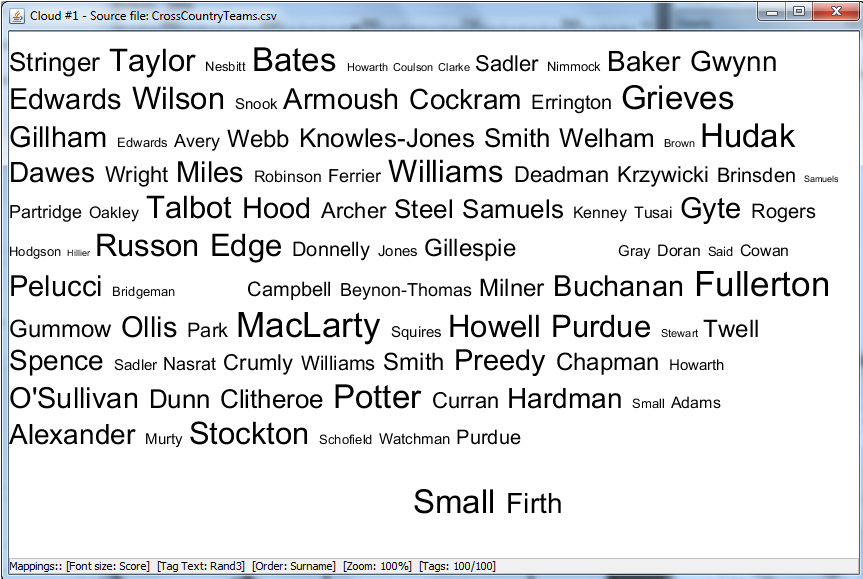
\includegraphics[scale=0.50]{mixedfont.png}
  \label{fig:mixedfont}
  \caption{\textit{Order and font size mappings are different}}
\end{subfigure}
  \caption{\textit{Cross country team members}}
  \label{fig:fontsize}
\end{figure}

If the ``Use tanh for mapping'' option is not selected, ratio field types are mapped linearly. ETC...

\subsection{Colour} \label{colourmappings}

\subsection{Transparency}


*********************************

\subsection{Goals}

Exploring quality assurance data such as metrics and code smells with a tag cloud visualisation system. Additionally, the possibility of software process management data and general multi-variate data.

Original prototype produced. Changes I made to it:

\begin{itemize}
\item usability improvements
\item ensure system copes with specific software engineering challenges identified (Chapter~\ref{chap:softvis})
\item changes resulting from tag cloud visual variable analysis (Chapter~\ref{chap:tagclouds})
\item improvements generated from heuristic evaluation (Chapter~\ref{chap:heuristiceval})
\end{itemize}

\subsection{Addressing the challenges specific to software engineering data}

\begin{itemize}
\item heavily skewed
\item contains outliers that may be important
\item large numbers of data points. scale
\item textual information. long identifiers
\item ensuring appropriate mappings
\end{itemize}

\subsection{Addressing the challenges specific to tag cloud visualisation}


\begin{itemize}
\item textual data - multiple word tags. Increased prominence of text (tag length visual variable).
\item Categorical data vs continuous data. Mapping changing, colour, legend.
\end{itemize}

\subsection{Mappings}

Ensuring the appropriate visual variables are selected for mapping purposed. Order, size, colour and transparency (in order of perceived usefulness, importance).


\begin{itemize}
\item tag length - filters applied
\item ordering
\item font size - limitations and constraints due to canvas size, reading ease
\item font family - familiar fonts for reading accuracy
\item font colour - divided into colour transparency and colour. Colour palettes. Background colour use by default.
\end{itemize}

\subsection{Bertin's visual variables}

Chosen mappings are selective and associative. Quantativive issues - comparisons using mouse drags.

\subsection{Tasks}

\begin{itemize}
\item Identify similar characteristics of data 
\item Identify data distribution 
\item Identify data correlations 
\item Detect outliers in a correlation
\item Finding minimum/maximum values
\item Comparison of data elements  
\item Discover trends 
\end{itemize}

% ------------------------------------------------------------------------


%%% Local Variables: 
%%% mode: latex
%%% TeX-master: "../thesis"
%%% End: 
